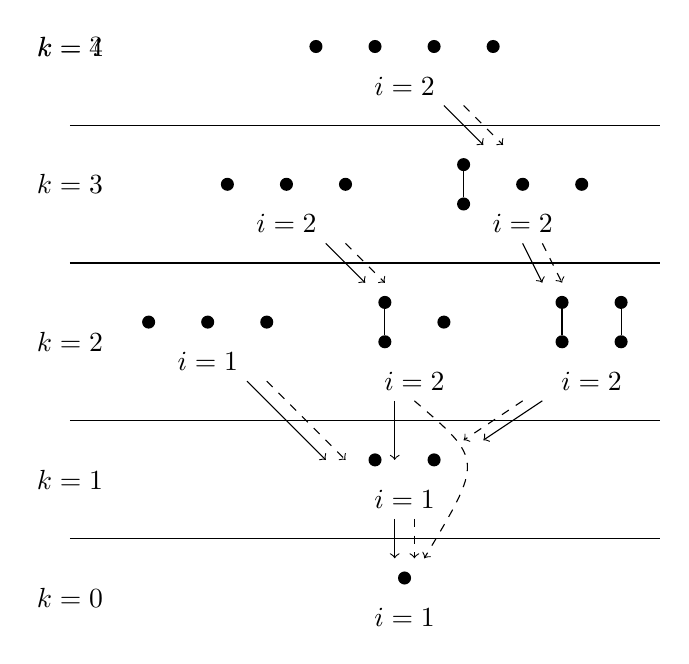
\begin{tikzpicture}

  % Level k = 4
  \uncover<1-3>{
    \node at (-1, 8) {$k=\text{ ?}$};
  }
  \uncover<4->{
    \node at (-1, 8) {$k=4$};
  }

  \node[circle,fill=black,scale=0.5] (k4_1) at (2.125 + 0 * 0.75, 8) {};
  \node[circle,fill=black,scale=0.5] (k4_2) at (2.125 + 1 * 0.75, 8) {};
  \node[circle,fill=black,scale=0.5] (k4_3) at (2.125 + 2 * 0.75, 8) {};
  \node[circle,fill=black,scale=0.5] (k4_4) at (2.125 + 3 * 0.75, 8) {};
  \node at (2.125 + 0.75 * 1.5, 7.5) {$i=2$};

  \uncover<4->{
    \draw[->, dashed] (4, 7.25) -- (4.5, 6.75);
    \draw[->] (3.75, 7.25) -- (4.25, 6.75);

    \draw (-1, 7) -- (6.5, 7);

    % Level k = 3
    \node at (-1, 6.25) {$k=3$};

    \node[circle,fill=black,scale=0.5] (k3_1) at (1 + 0 * 0.75, 6.25) {};
    \node[circle,fill=black,scale=0.5] (k3_2) at (1 + 1 * 0.75, 6.25) {};
    \node[circle,fill=black,scale=0.5] (k3_3) at (1 + 2 * 0.75, 6.25) {};
    \node at (1 + 0.75, 5.75) {$i=2$};

    \draw[->, dashed] (2.5, 5.5) -- (3, 5);
    \draw[->] (2.25, 5.5) -- (2.75, 5);

    \node[circle,fill=black,scale=0.5] (k3_4) at (4 + 0 * 0.75, 6.5) {};
    \node[circle,fill=black,scale=0.5] (k3_5) at (4 + 0 * 0.75, 6) {};
    \node[circle,fill=black,scale=0.5] (k3_6) at (4 + 1 * 0.75, 6.25) {};
    \node[circle,fill=black,scale=0.5] (k3_7) at (4 + 2 * 0.75, 6.25) {};
    \draw (k3_4) -- (k3_5);
    \node at (4 + 0.75, 5.75) {$i=2$};

    \draw[->, dashed] (5, 5.5) -- (5.25, 5);
    \draw[->] (4.75, 5.5) -- (5, 5);
  } \uncover<3->{

    \draw (-1, 5.25) -- (6.5, 5.25);

    % Level k = 2
    \node at (-1, 4.25) {$k=2$};

    \node[circle,fill=black,scale=0.5] (k2_1) at (0 + 0 * 0.75, 4.5) {};
    \node[circle,fill=black,scale=0.5] (k2_2) at (0 + 1 * 0.75, 4.5) {};
    \node[circle,fill=black,scale=0.5] (k2_3) at (0 + 2 * 0.75, 4.5) {};
    \node at (0 + 0.75, 4) {$i=1$};

    \draw[->, dashed] (1.5, 3.75) -- (2.5, 2.75);
    \draw[->] (1.25, 3.75) -- (2.25, 2.75);

    \node[circle,fill=black,scale=0.5] (k2_4) at (3 + 0 * 0.75, 4.25) {};
    \node[circle,fill=black,scale=0.5] (k2_5) at (3 + 0 * 0.75, 4.75) {};
    \node[circle,fill=black,scale=0.5] (k2_6) at (3 + 1 * 0.75, 4.5) {};
    \draw (k2_4) -- (k2_5);
    \node at (3 + 0.75 * 0.5, 3.75) {$i=2$};

    \draw[->, dashed] (3.375, 3.5) .. controls (4.25, 2.75) .. (3.5, 1.5);
    \draw[->] (3.125, 3.5) -- (3.125, 2.75);

    \node[circle,fill=black,scale=0.5] (k2_7) at (5.25 + 0 * 0.75, 4.25) {};
    \node[circle,fill=black,scale=0.5] (k2_8) at (5.25 + 0 * 0.75, 4.75) {};
    \node[circle,fill=black,scale=0.5] (k2_9) at (5.25 + 1 * 0.75, 4.25) {};
    \node[circle,fill=black,scale=0.5] (k2_10) at (5.25 + 1 * 0.75, 4.75) {};
    \draw (k2_7) -- (k2_8);
    \draw (k2_9) -- (k2_10);
    \node at (5.25 + 0.75 * 0.5, 3.75) {$i=2$};

    \draw[->, dashed] (4.75, 3.5) -- (4, 3);
    \draw[->] (5, 3.5) -- (4.25, 3);
  } \uncover<2->{

    \draw (-1, 3.25) -- (6.5, 3.25);
    % Level k = 1
    \node at (-1, 2.5) {$k=1$};

    \node[circle,fill=black,scale=0.5] (k1_1) at (2.875 + 0 * 0.75, 2.75) {};
    \node[circle,fill=black,scale=0.5] (k1_2) at (2.875 + 1 * 0.75, 2.75) {};
    \node at (2.875 + 0.75 * 0.5, 2.25) {$i=1$};

    \draw[->, dashed] (3.375, 2) -- (3.375, 1.5);
    \draw[->] (3.125, 2) -- (3.125, 1.5);
  }

  \draw (-1, 1.75) -- (6.5, 1.75);

  % Level k = 0
  \node at (-1, 1) {$k=0$};

  \node[circle,fill=black,scale=0.5] (k0_1) at (3.25, 1.25) {};
  \node at (3.25, 0.75) {$i=1$};
\end{tikzpicture}
